\documentclass[UTF8]{beamer}
\usepackage{ctex}
\usepackage{fontspec}
\usepackage{comment}
\usepackage{xeCJK}
\setCJKmainfont{KaiTi}
\setCJKmonofont{KaiTi}
\setCJKsansfont{Microsoft YaHei}
\usefonttheme{professionalfonts}
\usepackage{graphicx}
\graphicspath{{fig/}} % storage figure in a sub-folder
% \usepackage[parfill]{parskip} % Activate to begin paragraphs with an empty line rather than an indent
\usepackage{epstopdf}
\usepackage{bm}
\usepackage{nkcolor}
\usepackage{hyperref}
\hypersetup{CJKbookmarks=true}
\usepackage{url}
\usepackage{amsmath}
\usepackage{amsthm}
%\theoremstyle{definition}
%\newtheorem{theorem}{定理}
%\newtheorem{definition}{定义}
%\newtheorem{corollary}{推论}
%\newtheorem{example}{例}
\usepackage{booktabs} % for much better looking tables
\usepackage{cite} % reference
\usepackage{array} % for better arrays (eg matrices) in maths
%\usepackage{paralist} % very flexible & customisable lists (eg. enumerate/itemize, etc.)
\usepackage{verbatim} % adds environment for commenting out blocks of text & for better verbatim
\usepackage{subfig} % make it possible to include more than one captioned figure/table in a single float
% These packages are all incorporated in the memoir class to one degree or another...
%\usepackage{threeparttable}
\usepackage{cases} %equation set
\usepackage{multirow} %use table
\usepackage{enumerate}
\usepackage{algorithm}
\usepackage{algorithmic}
\usepackage{xcolor}
%\usepackage{capt-of}
\setcounter{tocdepth}{1}%只显示section,不显示subsection
\usepackage{listings}
\lstset{tabsize=4, keepspaces=true,
    xleftmargin=2em,xrightmargin=0em, aboveskip=1em,
    backgroundcolor=\color{gray!20},  % 定义背景颜色
    frame=none,                       % 表示不要边框
    extendedchars=false,              % 解决代码跨页时,章节标题,页眉等汉字不显示的问题
    numberstyle=\ttfamily,
    basicstyle=\ttfamily,
    keywordstyle=\color{blue}\bfseries,
    breakindent=10pt,
    identifierstyle=,                 % nothing happens
    commentstyle=\color{green}\small,  % 注释的设置
    morecomment=[l][\color{green}]{\#},
    numbers=left,stepnumber=1,numberstyle=\scriptsize,
    showstringspaces=false,
    showspaces=false,
    flexiblecolumns=true,
    breaklines=true, breakautoindent=true,breakindent=4em,
    escapeinside={/*@}{@*/},
}

\title[重庆大学]{Beamer模板\\Style of ChongQing University}
\author[吴昭]{吴昭\\(\url{lihua@163.com})}
\institute{重庆大学}
%\author[Calvin]{Calvin\inst{1} \and Cleven\inst{2}}
%\institute[Univ]{\inst{1}南开大学 \and \inst{2}克莱登大学}
\date{\today}


\begin{document}
%%%%%%%%%% 定理类环境的定义 %%%%%%%%%%
%% 必须在导入中文环境之后

\renewcommand{\contentsname}{目录}     % 将Contents改为目录
\renewcommand{\abstractname}{摘要}     % 将Abstract改为摘要
\renewcommand{\refname}{参考文献}      % 将References改为参考文献
\renewcommand{\indexname}{索引}
\renewcommand{\figurename}{图}
\renewcommand{\tablename}{表}
\renewcommand{\appendixname}{附录}
%\renewcommand{\proofname}{证明}
%\renewcommand{\algorithm}{算法}
%----------------------------------------------------------------------
% Title frame
\begin{frame}[plain]
\maketitle
\end{frame}

%----------------------------------------------------------------------
% Outline frame

\begin{frame}
\frametitle{目录}
\tableofcontents
\end{frame}


%%%%%%%%%%%%%%%%%%%%%%%%%%%%%%%%%%%%%%%%%%%%%%%%%%%%%%%%%%%%%%%%%

\section[Introduction ����]{Introduction}\label{sec:1}

%%%%%%%%%%%%%%%%%%%%%%%%%%%%%% ����Ŀ¼ҳ %%%%%%%%%%%%%%%%%%%%%%%%%%%%%%%%%%%

\begin{frame}%<beamer>
    \frametitle{\textsc{Contents}} \vspace{-1.05cm}
    \begin{multicols}{2}
    %\begin{figure}
    \begin{minipage}[t]{0.55\textwidth}
    \tableofcontents[currentsection,hideallsubsections]
    % [currentsection,hideallsubsections][sectionstyle=show/shaded,subsectionstyle=show/shaded/hide]
    \end{minipage}

    \begin{minipage}[t]{0.55\textwidth}
    \vspace{0.44cm}
    \begin{spacing}{1.2} % ������� ��Ҫ\usepackage{setspace}
    \begin{itemize}
    \item\hyperlink{subsec:1-1}{�������������}
    \item\hyperlink{subsec:1-2}{����취}
    %\item\hyperlink{subsec:1-3}{Symbols and Notes}
    %\item\hyperlink{subsec:1-4}{EM Spectrum}
    \end{itemize}
    \end{spacing}
    \end{minipage}
    %\end{figure}
    \end{multicols}

\end{frame}

%%%%%%%%%%%%%%%%%%%%%%%%%%%%%%%%%%%%%%%%%%%%%%%%%%%%%%%%%%%%%%%%%
\subsection[History and background]{����������}\label{subsec:1-1}
%%%%%%%%%%%%%%%%%%%%%%%%%%%%%%%%%%%%%%%%%%%%%%%%%%%%%%%%%%%%%%%%%
\begin{frame}
\frametitle{\textsc{����, ����}}%\transsplitverticalin

\begin{itemize}
\hilite<1>\item ���Բ���ϵ: ʹţ����ѧ�����IJ���ϵ\pause

\hilite<2>\item ţ����ѧ��ʱ�չ�: ٤���Ա任
\begin{align}
&t'=t,\\
&x'=x+vt,\\
&y'=y,\\
&z'=z.\pause
\end{align}
%\begin{figure}
 % \begin{center}
  %  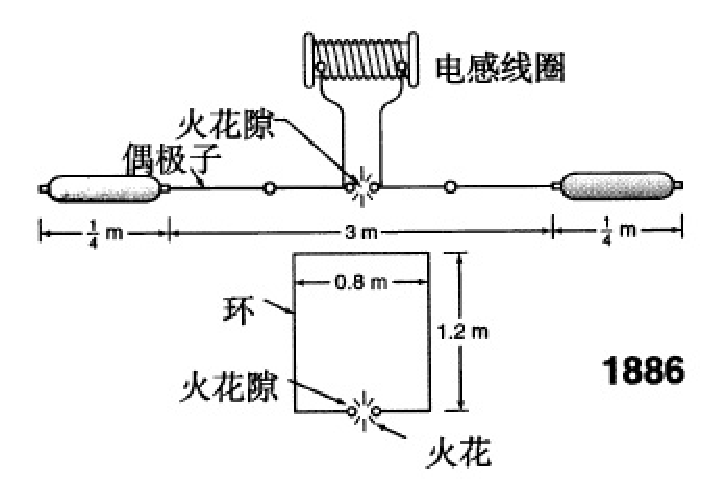
\includegraphics[scale=0.4]{ch1/first_radio_link} % ͼƬ�������Դ�Щ��ĸ��ͷ
  %\end{center}
%\end{figure}

\hilite<3>\item ٤���������ԭ��: %ţ����ѧ����, ��һ�й���ϵ�任����.

\end{itemize}

\end{frame}

%%%%%%%%%%%%%%%%%%%%%%%%%%%%%%%%%%%%%%%%%%%%%%%%%%%%%%%%%%%%%%%%%
\begin{frame}
\frametitle{\textsc{History}} % \transsplitverticalout

\begin{itemize}
    \hilite<1>\item ����ϵ����\pause
    \hilite<2>\item �ٶ����������\pause
    \hilite<3>\item ��Ų�: ������������, ��������
\begin{align}\left.
\begin{array}{l}
\nabla\cdot\bm{E}=\frac{\rho}{\epsilon_0}\\
\nabla\times\bm{B}=\mu_0\bm{J}+\mu_0\epsilon_0\frac{\partial\bm{E}}{\partial t},\\
\nabla\cdot\bm{B}=0\\
\nabla\times\bm{E}=-\frac{\partial\bm{B}}{\partial t}\end{array}
\right\}\bm{E}=\bm{E}_0\cos(kx-\omega t),
\end{align}
\begin{align}
c=\frac{\omega}{k}=\frac{1}{\sqrt{\mu_0\epsilon_0}}\nonumber
\end{align}
   % \begin{figure}
    %\begin{center}
     %   \includegraphics[scale=0.5]{ch1/antenna_marconi} % ͼƬ�������Դ�Щ��ĸ��ͷ
    %\end{center}
    %\end{figure}
\end{itemize}
%\rightline{\hyperlink{sec:1}{\beamerreturnbutton{back}} }

\end{frame}

%%%%%%%%%%%%%%%%%%%%%%%%%%%%%%%%%%%%%%%%%%%%%%%%%%%%%%%%%%%%%%%%%
\subsection[���]{�������}\label{subsec:1-2}
%%%%%%%%%%%%%%%%%%%%%%%%%%%%%%%%%%%%%%%%%%%%%%%%%%%%%%%%%%%%%%%%%

\begin{frame}
\frametitle{\textsc{��ν��?}}%\transwipe % ͿĨЧ��

\begin{itemize}% [<+-| structure@+>]
\hilite<1>\item ���ٲ���ԭ��\pause

%\hilite<2>\item 1960s-1990s, advances made in computer architecture
%and technology have had a major impact on the advance of modern
%antenna technology, numerical methods were introduced that allowed
%previously intractable complex antenna system configurations to be
%analyzed and designed very accurately.
\hilite<2>\item ���������ԭ��: һ�����������ڲ�ͬ����ϵ����ʽ��ͬ
\end{itemize}
%\rightline{\hyperlink{sec:1}{\beamerreturnbutton{back}} }

\end{frame}

%%%%%%%%%%%%%%%%%%%%%%%%%%%%%%%%%%%%%%%%%%%%%%%%%%%%%%%%%%%%%%%%%

\section[�����ʱ�չ۵ļ��з�ӳ: �����ȱ任]{Lorentz transformation} %[���У������]

%%%%%%%%%%%%%%%%%%%%%%%%%%%%%% ����Ŀ¼ҳ %%%%%%%%%%%%%%%%%%%%%%%%%%%%%%%%%%%

\begin{frame}%<beamer>
    \frametitle{\textsc{Contents}} \vspace{-0.85cm}\label{sec:2}
    \begin{multicols}{2}
    \begin{minipage}[t]{0.55\textwidth}
    \tableofcontents[currentsection,hideallsubsections]
    % [currentsection,hideallsubsections][sectionstyle=show/shaded,subsectionstyle=show/shaded/hide]
    \end{minipage}

    \begin{minipage}[t]{0.55\textwidth}
    \vspace{0.5cm}
    \begin{spacing}{0.9} % ������� ��Ҫ\usepackage{setspace}
    \begin{itemize}
        \item\hyperlink{subsec:2-1}{���ٲ����Ե��¼��������}
        \item\hyperlink{subsec:2-2}{�ɼ������, ���������ȱ任}
       % \item\hyperlink{subsec:2-3}{��������, ��~``��'' �ӻ�}
       % \item\hyperlink{subsec:2-4}{Directivity and Gain}
        %\item\hyperlink{subsec:2-5}{Antenna Apertures}
        %\item\hyperlink{subsec:2-6}{Radio Communication Link}
        %\item\hyperlink{subsec:2-7}{Fields From Dipole}
        %\item\hyperlink{subsec:2-8}{Antenna Field Zones}
        %\item\hyperlink{subsec:2-9}{Shape-Impedance Considerations}
        %\item\hyperlink{subsec:2-10}{Polarization}
    \end{itemize}
    \end{spacing}
    \end{minipage}
    \end{multicols}
\end{frame}

%%%%%%%%%%%%%%%%%%%%%%%%%%%%%%%%%%%%%%%%%%%%%%%%%%%%%%%%%%%%%%%%%
\subsection[���ٲ����Ե��¼��������]{���������}\label{subsec:2-1}
%%%%%%%%%%%%%%%%%%%%%%%%%%%%%%%%%%%%%%%%%%%%%%%%%%%%%%%%%%%%%%%%%

\begin{frame}
\frametitle{\textsc{�¼�, �ɹ��ź���ϵ�ŵ��¼�}}% \transblindshorizontal % ˮƽ����Ч��

\begin{itemize}
\hilite<1>\item �¼�~$(ct,x,y,z)$. �����ɹ���ϵ�ŵ��¼�, ��~$\Sigma$ ��~$\Sigma'$ �зֱ���
\begin{align}
c^2t^2-x^2-y^2-z^2=0=c^2t'^2-x'^2-y'^2-z'^2.\pause
\end{align}

\hilite<2>\item һ�������, $c^2t^2-x^2-y^2-z^2\neq0$, then what is the relationship between them?
\pause

\hilite<3>\item So we still have
\begin{align}
c^2t^2-x^2-y^2-z^2=c^2t'^2-x'^2-y'^2-z'^2.\nonumber\\\nonumber
\end{align}
\end{itemize}


\end{frame}

%%%%%%%%%%%%%%%%%%%%%%%%%%%%%%%%%%%%%%%%%%%%%%%%%%%%%%%%%%%%%%%%%

\begin{frame}
\frametitle{\textsc{ij���ռ�������Ҫ�IJ�����/����: ���}}


\begin{itemize}

\hilite<1>\item ��Ϊ~$c^2t^2-x^2-y^2-z^2$ ������������ԡ���Ҫ��, ���ǽ����������, �м��, ��Ϊ
\begin{align}
ds^2=c^2dt^2-dx^2-dy^2-dz^2.\pause
\end{align}

\hilite<2>\item ���ʸ��~$x^\mu=(ct,x,y,z)$,

Э��ʸ��~$x_\mu=(ct,-x,-y,-z)$,
\pause

\hilite<3>\item �������ǿɵ�
\begin{align}
ds^2=dx^\mu dx_\mu.\nonumber
\end{align}
\end{itemize}







\end{frame}

%%%%%%%%%%%%%%%%%%%%%%%%%%%%%%%%%%%%%%%%%%%%%%%%%%%%%%%%%%%%%%%%%
\begin{frame}
\frametitle{\textsc{��ͬʱ�վ��в�ͬ�Ķȹ�}}

\begin{itemize}

\hilite<1>\item �����������¶��׶Գ�����
\begin{align}
g_{\mu\nu}=\left[
\begin{array}{cccc}
1&0&0&0\\
0&-1&0&0\\
0&0&-1&0\\
0&0&0&-1
\end{array}
\right],
\end{align}
��Ϊ�ȹ�,\pause

\hilite<2>\item �Ϳɽ������һ����Ϊ
\begin{align}
ds^2=g_{\mu\nu}dx^\mu dx^\nu.\nonumber\pause
\end{align}


\hilite<3>\item �ȹ��ڹ����������, ���и���Ҫ������.
\end{itemize}



\end{frame}


%%%%%%%%%%%%%%%%%%%%%%%%%%%%%%%%%%%%%%%%%%%%%%%%%%%%%%%%%%%%%%%%%
\subsection[�ɼ������, ���������ȱ任]{�ɼ�����䵼�������ȱ任}\label{subsec:2-2}
%%%%%%%%%%%%%%%%%%%%%%%%%%%%%%%%%%%%%%%%%%%%%%%%%%%%%%%%%%%%%%%%%

\begin{frame}
\frametitle{\textsc{�¼��任��һ���ϵ}}

\begin{itemize}

\hilite<1>\item �򵥷���, ���ѵ�֪, ������������ϵ�п�ͬһ���¼��������ϵΪ
\begin{align}
ct'=&act+bx,\\
x'=&Act+Bx,\\
y'=&y,\\
z'=&z.\pause
\end{align}


\hilite<2>\item ���ü��������~$c^2t'^2-x'^2=c^2t^2-x^2$, ����
\begin{align}
\left.\begin{array}{c}
a^2-A^2=1\\
b^2-B^2=-1\\
ab-AB=0
\end{array}
\right\}\Rightarrow
\left\{\begin{array}{c}
a=B,A=b,\\
a^2-b^2=1.
\end{array}\right.\nonumber
\end{align}
\end{itemize}



\end{frame}

%%%%%%%%%%%%%%%%%%%%%%%%%%%%%%%%%%%%%%%%%%%%%%%%%%%%%%%%%%%%%%%%%

\begin{frame}
\frametitle{\textsc{�����ȱ任}}
\begin{itemize}

\hilite<1>\item ��ǰ�����, �ɽ��任��һ��������
\begin{align}
ct'=&act+bx,\\
x'=&bct+ax;
\end{align}
ע������~$a^2-b^2=1$.\pause

\hilite<2>\item $\Sigma'$ �п��Լ�ԭ��������Ϊ~$0$, $\Sigma$ �п�����~$-vt$, ����������
\begin{align}
0=bct-avt;
\end{align}
��
\begin{align}
\frac{b}{a}=\frac{v}{c}:=\beta.\nonumber
\end{align}
\end{itemize}


\end{frame}

%%%%%%%%%%%%%%%%%%%%%%%%%%%%%%%%%%%%%%%%%%%%%%%%%%%%%%%%%%%%%%%%%

\begin{frame}
\frametitle{\textsc{�����ȱ任}}
\begin{itemize}

\hilite<1>\item ��ǰ�����, �������ս��
\begin{align}
a=&\frac{1}{\sqrt{1-\frac{v^2}{c^2}}}:=\gamma,\\
b=&\frac{v/c}{\sqrt{1-\frac{v^2}{c^2}}}=\beta\gamma.
\end{align}

\end{itemize}


\end{frame}



\begin{frame}
\frametitle{\textsc{�����ȱ任}}
\begin{itemize}


\hilite<1>\item So at last, we get the final form of the Lorentz transformation:
\begin{equation}
\left\{
\begin{aligned}
ct'&=\frac{ct+\frac{v}{c}x}{\sqrt{1-\frac{v^2}{c^2}}},\\
x'&=\frac{vt+x}{\sqrt{1-\frac{v^2}{c^2}}},\\
y'&=y,\\
z'&=z;\pause
\end{aligned}
\right.
\end{equation}

\hilite<2>\item Lorentz boost.%�����任��ͬһ�¼��ڲ�ͬ����ϵ�еı任ʽ, ���Ϊ�����ȱ任��~$x$ �����ϵ�~boost.




\end{itemize}


\end{frame}





\begin{frame}
\frametitle{\textsc{�����ȱ任}}
\begin{itemize}


\hilite<1>\item ���ǻ��ɽ������任�þ�����ʽ��Ϊ
\begin{align}
\left[
\begin{array}{l}
ct'\\x'\\y'\\z'
\end{array}
\right]=
\left[
\begin{array}{cccc}
\gamma&\beta\gamma&0&0\\
\beta\gamma&\gamma&0&0\\
0&0&1&0\\
0&0&0&1
\end{array}
\right]
\left[
\begin{array}{l}
ct\\x\\y\\z
\end{array}
\right];
\end{align}
\end{itemize}

%\rightline{\hyperlink{sec:2}{\beamerreturnbutton{back}} }
\end{frame}


%%%%%%%%%%%%%%%%%%%%%%%%%%%%%%%%%%%%%%%%%%%%%%%%%%%%%%%%%%%%%%%%%

\section[��������۵�ʱ�չ�]{spacetime of SR}

%%%%%%%%%%%%%%%%%%%%%%%%%%%%%% ����Ŀ¼ҳ %%%%%%%%%%%%%%%%%%%%%%%%%%%%%%%%%%%

\begin{frame}%<beamer>
    \frametitle{\textsc{Contents}} \vspace{-0.85cm}\label{sec:3}
    \begin{multicols}{2}
    \begin{minipage}[t]{0.55\textwidth}
    \tableofcontents[currentsection,hideallsubsections]
    % [currentsection,hideallsubsections][sectionstyle=show/shaded,subsectionstyle=show/shaded/hide]
    \end{minipage}

    \begin{minipage}[t]{0.55\textwidth}
    \vspace{0.6cm}
    \begin{spacing}{0.9} % ������� ��Ҫ\usepackage{setspace}
    \begin{itemize}
        \item\hyperlink{subsec:3-1}{��������, ��������; ��~``��'' �ӻ�, ����������}
        \item\hyperlink{subsec:3-2}{ʱ��ͼ, �����, ͬʱ�������}
        \item\hyperlink{subsec:3-3}{�ִ����澡ͷ; ���ȥ����δ���˻���}
      %  \item\hyperlink{subsec:3-4}{Waveguide Antennas}
      %  \item\hyperlink{subsec:3-5}{Flat-Sheet Reflector Antennas}
      %  \item\hyperlink{subsec:3-6}{Radio Communication Link}
      %  \item\hyperlink{subsec:3-7}{Fields From Dipole}
      %  \item\hyperlink{subsec:3-8}{Antenna Field Zones}
      %  \item\hyperlink{subsec:3-9}{Shape-Impedance Considerations}
    \end{itemize}
    \end{spacing}
    \end{minipage}
    \end{multicols}
\end{frame}

%%%%%%%%%%%%%%%%%%%%%%%%%%%%%%%%%%%%%%%%%%%%%%%%%%%%%%%%%%%%%%%%%
\subsection[��������]{shorter and slower}\label{subsec:3-1}
%%%%%%%%%%%%%%%%%%%%%%%%%%%%%%%%%%%%%%%%%%%%%%%%%%%%%%%%%%%%%%%%%


\begin{frame}
\frametitle{\textsc{��������}}
\begin{itemize}

\hilite<1>\item �����ȱ任, ��ʹ���Ƿ���һ��ȫ�µ������; ͬʱ, ����������ͬʱ���һ��, ������һ�θ���̵ؾ�������: �й������Ǵ�dz��, ����ȷ�Ĺ��������ڸ���ȷ������Ļ��.\pause

\hilite<2>\item ���Ǽ���, $\Sigma'$ ϵ����һ����, ��Ϊ~$L'$, ��, ��~$\Sigma$ �Ͽ���, ����~$L$ �Ƕ���?
\begin{align}
x'_1=\gamma\beta ct+\gamma x_1,\\
x'_2=\gamma\beta ct+\gamma x_2,
\end{align}
��ʽ�������
\begin{align}
L'=\gamma L, or~L=\sqrt{1-\frac{v^2}{c^2}}L'.\nonumber
\end{align}

\end{itemize}

\end{frame}

%%%%%%%%%%%%%%%%%%%%%%%%%%%%%
\begin{frame}
\frametitle{\textsc{���ڳ��ȵļ�������}}
\begin{itemize}

\hilite<1>\item ���⵽���ܲ���װ�³���? ���������ͬʱ/��ͬʱ��;\pause 

\hilite<2>\item �������׻᲻����±���? �����ij��������� (�������������һֱ��, ����ͬ); ����ͬʱ/��ͬʱ��;\pause

\hilite<3>\item ��·���׻᲻�ᱻ��ͨ? �⴫����ʱ��;\pause
\hilite<4>\item DZˮͧ���ϸ������³�? ����ȫ���Ļ���������, �޸���; ������~(������׹�����): ����������, ���ɴ���ˮ���������˶�������, ���ٴ��еķɴ�, ˮ��������������, �������ɲ�����������. ǰ��˵��, �д���ȶ. �����������������, ���Կ�����˲ʱ��. ʵ�����, ˮ��ͧ�ƶ��²����α�����, ����������; ��ˮ������ˮ�������, ����˼����, �ƿ���֮ˮ/�谭��, ȴ���ܵ��κη�����, �������. ���Լ����������ˮ (��ѹ����ը), Ҳ���������������ƶ�.
\end{itemize}

\end{frame}

%%%%%%%%%%%%%%%%%%%%%%%%%%%%%%%%%%%%%%%%%%%%%%%%%%%%%%%%%%%%%%%%%


\begin{frame}
\frametitle{\textsc{��~``��'' �ӻ�, ����������}}
\begin{itemize}

\hilite<1>\item ���Ǽ�����~$\Sigma$ ϵ��ij�̶��㴦, ����һ�ν���, ������, ����
\begin{align}
ct'_1=\gamma ct_1+\beta\gamma x,\\
ct'_2=\gamma ct_2+\beta\gamma x,
\end{align}
������֪
\begin{align}
\Delta t'=\gamma \Delta t.\pause
\end{align}


\hilite<2>\item ����˭������, ˭����?\pause
\hilite<3>\item ˫���ű�ը����: �᲻��ը?

\end{itemize}

%\rightline{\hyperlink{sec:3}{\beamerreturnbutton{back}} }

\end{frame}


%%%%%%%%%%%%%%%%%%%%%%%%%%%%%%%%%%%%%%%%%%%%%%%%%%%%%%%%%%%%%%%%%








%%%%%%%%%%%%%%%%%%%%%%%%%%%%%%%%%%%%%%%%%%%%%%%%%%%%%%%%%%%%%%%%%
\subsection[ʱ��ͼ, �����, ͬʱ�������]{causality}\label{subsec:3-2}
%%%%%%%%%%%%%%%%%%%%%%%%%%%%%%%%%%%%%%%%%%%%%%%%%%%%%%%%%%%%%%%%%

% \begin{frame}
% \frametitle{\textsc{(ij�¼���) ʱ��ͼ, ��׶}}
% \begin{figure}[!h]
% \begin{center}
% 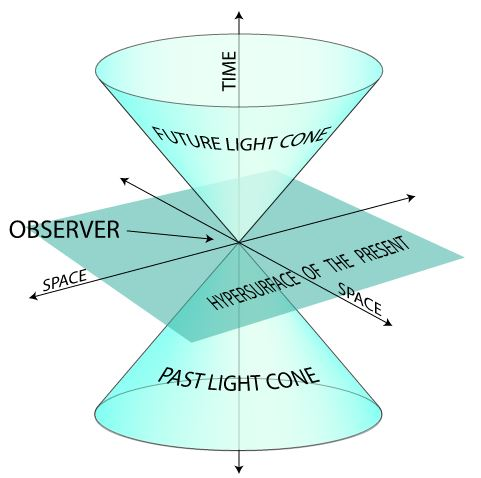
\includegraphics[width=4.3 cm]{figure/space.jpg}
% \caption{���/ʱ������Ļ���.}
% \label{space}
% \end{center}
% \end{figure}
% \end{frame}


\begin{frame}
\frametitle{\textsc{�������¼���ij�¼��ļ���ķ���}}
\begin{itemize}
\hilite<1>\item �����~$ds^2=0$, ��׶��\pause
\hilite<2>\item ��ʱ���~$ds^2>0$, ��׶��: ����δ��, ���Թ�ȥ\pause
\hilite<3>\item ��ռ��~$dx^2<0$, ��׶��: �ص�δ��, ͻ�����?
\end{itemize}
\end{frame}


\begin{frame}
\frametitle{\textsc{�����, ��������}}
\begin{itemize}
\hilite<1>\item ����ɲ�����: �������ϵ���´���ز��ɱ�; ͬʱ���\pause
\hilite<2>\item ��ά������ά�����۲�: ����, ʱ�����\pause
\hilite<3>\item ��ά�������, ��ά����ʸ��, ��ά�ٶ�/����ʸ��, ����.
\end{itemize}
%\rightline{\hyperlink{sec:3}{\beamerreturnbutton{back}} }
\end{frame}




%%%%%%%%%%%%%%%%%%%%%%%%%%%%%%%%%%%%%%%%%%%%%%%%%%%%%%%%%%%%%%%%%
\subsection[�ִ����澡ͷ; ���ȥ����δ���˻���]{niubi}\label{subsec:3-3}
%%%%%%%%%%%%%%%%%%%%%%%%%%%%%%%%%%%%%%%%%%%%%%%%%%%%%%%%%%%%%%%%%

\begin{frame}
\frametitle{\textsc{�ִ����澡ͷ; ���ȥ����δ���˻���}}
�ִ����澡ͷ; ���ȥ����δ���˻���

\rightline{\hyperlink{sec:3}{\beamerreturnbutton{back}} }
\end{frame}

\section{总结与展望}

\begin{frame}{结论}
    \begin{description}
        \item[I] First of all
        \item[II] Besides
        \item[III] Last but not least
    \end{description}
\end{frame}




\end{document}

